
\section{Experimental Study} 
\label{sec:exp}

\todo{Detail the experimental setup used to test the different algorithms. Present the results in an understandable manner (graphics, tables, etc.). Draw conclusions about what things worked (and why) and which didn't (and why).  \ldots}


For every evaluation is first of all a table with all there parameter settings. Additionally there are the average winning rate and the standard deviation listed.
All the results are also visualized by boxplots. There you can see the minimum and maximum average wins overall iterations. Furthermore the blue rectangle shows 
the qartile values. The red line in the middle is the median and the blue dot is the mean (average wins).
Do not mix quartiles with the standard deviation that is something completely different.

In the following sections each of the approaches is evaluated. 

\todo{combinations really failed. explain it.}
\todo{why we use this parameters??? something is missing...why not an exhaustive search for finding the best parameter..no time? 
to less computational power...}

\subsection{Heuristic based Algorithm} 

The heuristic based algorithm has several parameter that changes the behaviour of the agent (figure~\ref{fig:heur}).
Firstly we just changed the maximal states field that provides a limit for saved states at
the AStar algorithm. As you can see the average winning rate increases by changing to a higher maximal states limit up to 20.
But if the variable is set to 25 we had a worse result. This might be that if this value is to low the target is not found 
by the AStar algorithm. Moreover if it is to large to many states are saved and we get trouble with the memory or the
garbage collector.


\begin{table}[htbp]
\center
\begin{tabular}{*9c}  \hline
\multicolumn{1}{p{1cm}}{\centering ID} & 
\multicolumn{1}{p{2cm}}{\centering Max.\\ States} & 
\multicolumn{1}{p{2cm}}{\centering Safety\\ Strategy} & 
\multicolumn{1}{p{2cm}}{\centering Safety\\ Iterations} & 
\multicolumn{1}{p{1cm}}{\centering Avg\\ Wins	} & 
\multicolumn{1}{p{1cm}}{\centering Std of Wins} \\ \hline
1 & 5 & SafetyAdvance & 5 & 0.517 & 0.0257099203 \\ \hline
2 & 15 & SafetyAdvance & 5 & 0.529 & 0.0197230829 \\ \hline
3 & 20 & SafetyAdvance & 5 & \textbf{0.532} & 0.0271293199 \\ \hline
4 & 25 & SafetyAdvance & 5 & 0.521 & 0.0192093727 \\ \hline
5 & 20 & SafetyGridSearch & - & 0.498 & 0.0235796522 \\ \hline
6 & 20 & SafetyIntelligent & 5 & 0.527 & 0.0184661853 \\ \hline
\end{tabular}
\label{fig:heur}
\caption{results of the heuristic based algorithms}
\end{table}

After that we tried to change the safety strategy to the grid and the intelligent search. Both results
are worse than the SafetyAdvance Strategy. Since the SafeGridSearch highly depends on the Explorer and the
classification of the object this might be the cause.
With the SafetyIntelligent we got no further improvement but it is nearly good as the SafetyAdvance approach.


\begin{figure}
\centering
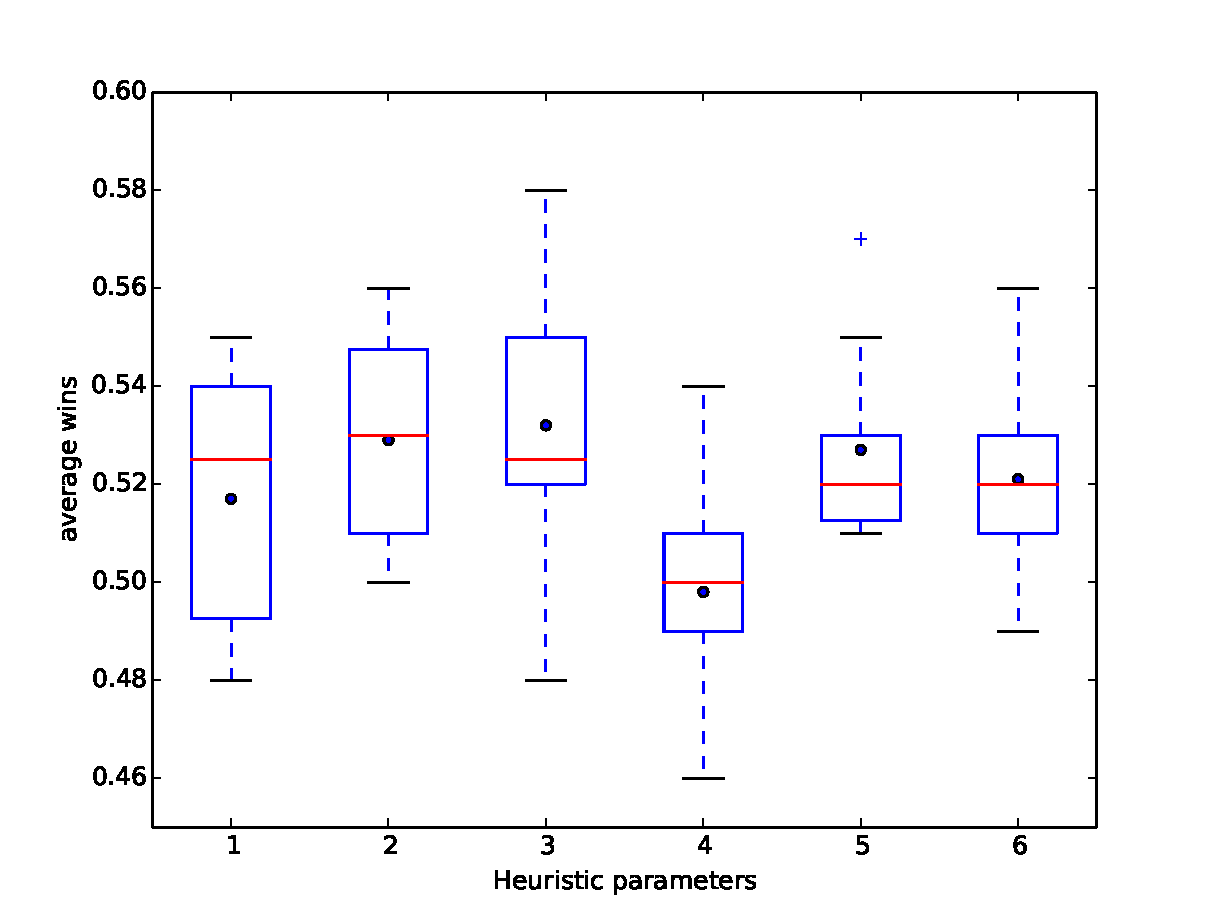
\includegraphics[scale=0.6]{images/eval_heur.pdf}
\caption{boxplot of the heuristic based algorithms}
\label{fig:eval_heur}
\end{figure}

The boxplot (figure~\ref{fig:eval_heur}) visualizes the quartiles. The best parameter setup has also the largest
quartile range. When you look at the table also the largest standard deviation (which doesn't have to be the same).
If the target is not found the agent is staying alive. The risk of a longer search to reach a simulation state
that collides with the target could be the reason for the higher variance of the results.



\subsection{MCTS} 
We also tried to combine several approaches for example using the heuristic explorer 
for a better mcts iteration. 


\subsection{Evolutionary Algorithm} 

For the evolutionary algorithm we had a set up with different parameters.

\begin{table}[H]
\center
\caption{}
\begin{tabular}{*9c}  \hline
\multicolumn{1}{p{1cm}}{\centering ID} & 
\multicolumn{1}{p{2cm}}{\centering Safety\\ Iterations} & 
\multicolumn{1}{p{1cm}}{\centering Path Length} & 
\multicolumn{1}{p{1cm}}{\centering Size of\\ Pop.} & 
\multicolumn{1}{p{1cm}}{\centering Fittest\\ Pop.} & 
\multicolumn{1}{p{1cm}}{\centering Dyn. Path\\ Length} & 
\multicolumn{1}{p{1cm}}{\centering Min. Gen.} & 
\multicolumn{1}{p{1cm}}{\centering Avg\\ Wins	} & 
\multicolumn{1}{p{1cm}}{\centering Std of Wins} \\ \hline
1 & 2 & 6 & 14 & 5 & no & - & 0.459 & 0.023 \\ \hline
2 & 4 & 6 & 10 & 4 & no & - & 0.458 & 0.024 \\ \hline
3 & 5 & 4 & 14 & 5 & no & - & 0.466 & 0.028 \\ \hline
4 & 5 & 6 & 10 & 5 & no & - & 0.459 & 0.032 \\ \hline
5 & 5 & 6 & 13 & 4 & yes & 5 & 0.451 & 0.041 \\ \hline
6 & 5 & 6 & 14 & 3 & no & - & 0.471 & 0.018 \\ \hline
7 & 5 & 6 & 14 & 5 & no & - & 0.461 & 0.025 \\ \hline
8 & 5 & 6 & 14 & 5 & yes & 2 & 0.479 & 0.021 \\ \hline
9 & 5 & 6 & 14 & 5 & yes & 4 & 0.463 & 0.027 \\ \hline
10 & 5 & 6 & 14 & 5 & yes & 6 & 0.449 & 0.041 \\ \hline
11 & 5 & 6 & 14 & 7 & no & - & 0.474 & 0.028 \\ \hline
12 & 5 & 6 & 18 & 5 & no & - & 0.462 & 0.035 \\ \hline
13 & 5 & 8 & 14 & 5 & no & - & 0.453 & 0.029 \\ \hline
14 & 8 & 6 & 14 & 5 & no & - & 0.477 & 0.022 \\ \hline
\end{tabular}
\label{ea_result}
\end{table}



\begin{figure}
\centering
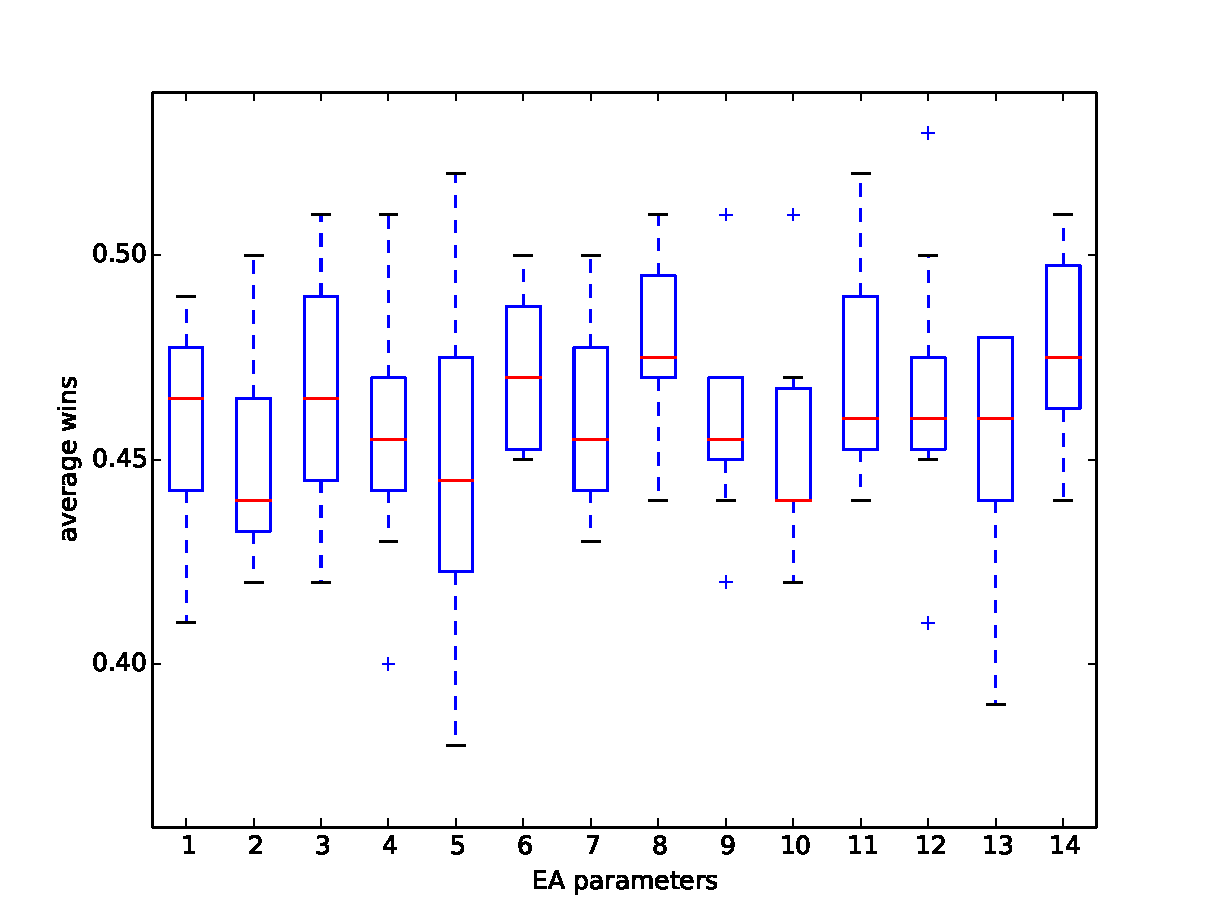
\includegraphics[scale=0.7]{images/eval_evolutionary.pdf}
\caption{result of the evolutionary algorithms}
\label{fig:eval_evo}
\end{figure}








\subsection{Evaluation of all approaches} 

